\documentclass[11pt,a4paper]{article}
\usepackage[utf8]{inputenc}
\usepackage[T1]{fontenc}
\usepackage[margin=2.3cm]{geometry}
\usepackage{amsmath,amssymb,amsthm,mathtools}
\usepackage{tikz}
\usetikzlibrary{quantikz2}
\usepackage{xcolor}
\usepackage{enumitem}
\usepackage{cancel}
\usepackage{hyperref}

% --- Dirac notation ---
\renewcommand{\ket}[1]{\left|#1\right\rangle}
\renewcommand{\bra}[1]{\left\langle#1\right|}
\renewcommand{\braket}[2]{\left\langle#1\middle|#2\right\rangle}
\newcommand{\ketbra}[2]{\left|#1\right\rangle\!\left\langle#2\right|}
\newcommand{\expval}[3]{\left\langle#1\middle|#2\middle|#3\right\rangle}
\newcommand{\Ket}[1]{\left|#1\right\rangle}
\newcommand{\Tr}{\operatorname{Tr}}
\newcommand{\Hil}{\mathcal{H}}
\newcommand{\CC}{\mathbb{C}}
\newcommand{\id}{\mathbb{I}}

% Marker for passages where the handwriting was hard to read
\newcommand{\CHECK}[1]{\textcolor{red}{[\textbf{CHECK:} #1]}}

\setlength{\parindent}{0pt}
\setlength{\parskip}{0.5em}

\title{QIP 1 -- Riassunto}
\author{}
\date{}

\begin{document}
\maketitle
\tableofcontents
\newpage

%======================================================================
\section{No-cloning theorem}

Suppose we want to copy a state $\ket{\psi}$: we want an operation that maps
\[
\ket{\psi}\otimes\ket{0} \longmapsto \ket{\psi}\otimes\ket{\psi}
= \alpha^2\ket{00} + \beta^2\ket{11} + \alpha\beta\ket{01} + \alpha\beta\ket{10}.
\]
A CNOT works for $\ket{\psi} = \ket{0},\ket{1}$ (similarly, the CNOT with control and target swapped, with the second qubit prepared in $\ket{+}$, copies $\ket{+},\ket{-}$), but doesn't work for a general $\ket{\psi} = \alpha\ket{0}+\beta\ket{1}$:
\[
\mathrm{CNOT}\bigl(\ket{\psi}\otimes\ket{0}\bigr) = \alpha\ket{00} + \beta\ket{11} \neq \ket{\psi}\otimes\ket{\psi}.
\]

\begin{itemize}
  \item For a set $S$ of quantum states, suppose there exists a unitary operation $U$ which maps
  $\ket{\psi}\otimes\ket{0} \mapsto \ket{\psi}\otimes\ket{\psi}$ $\forall \ket{\psi}\in S$\\
  $\Rightarrow$ the states in $S$ are mutually orthogonal.
\end{itemize}

%======================================================================
\section{Deutsch algorithm}

Consider a function $f:\{0,1\}\to\{0,1\}$. There are 4 such functions, 2 of which give constant output.
\begin{itemize}
  \item Given a black-box implementation of $f$, decide if $f$ is constant.
  \begin{itemize}
    \item[$\to$] \textsc{Classical}: 2 queries
    \item[$\to$] \textsc{Quantum}: 1 query
  \end{itemize}
\end{itemize}

We have $U_f$: $U_f\bigl(\ket{x}\otimes\ket{y}\bigr) = \ket{x}\otimes\ket{f(x)\oplus y}$
\begin{itemize}[label=--]
  \item $U_f\bigl(\ket{x}\otimes\ket{-}\bigr) = (-1)^{f(x)}\ket{x}\otimes\ket{-}$
  \item $U_f\bigl(\ket{+}\otimes\ket{-}\bigr) = (-1)^{f(0)}\frac{1}{\sqrt2}\bigl(\ket{0} + (-1)^{f(0)\oplus f(1)}\ket{1}\bigr)\otimes\ket{-}$
\end{itemize}
$\Rightarrow$ If $f$ constant, we have $\ket{+}\ket{-}$. If $f$ balanced, $\ket{-}\ket{-}$.\\
We can use $H$ to rotate back to the computational basis:
\begin{center}
\begin{quantikz}
\lstick{$\ket0$} & \gate{H} & \gate[2]{U_f} & \gate{H} & \meter{} & \setwiretype{c} \rstick{$= s$}\\
\lstick{$\ket1$} & \gate{H} & & & &
\end{quantikz}
\qquad
$s = \begin{cases} 0 \to \text{constant}\\ 1 \to \text{balanced}\end{cases}$
\end{center}

%======================================================================
\section{Postulates of QM}

\begin{enumerate}
  \item To each d.o.f.\ (\textsc{quantum system}) is associated a Hilbert space $\Hil \simeq \CC^d$ with inner product
  \[
  \braket{u}{v} = \sum_{j=1}^d u_j^* v_j \qquad \forall u,v\in\Hil.
  \]
  \item Physical observables are Hermitian operators on $\Hil$.
  \item The state of a quantum system is given by a normalized vector in $\Hil$.
  \item A measurement of $\hat A$ on system $S$ results in a single value of the set of the eigenvalues of $\hat A$.\\
  Let $\Pi_a$ be the projection operator onto the subspace of $\ket{\phi}$: $A\ket{\phi} = a\ket{\phi}$
  \[
  \Rightarrow \text{Born rule:}\quad P(a) = \expval{\psi}{\Pi_a}{\psi}, \qquad \langle A\rangle = \expval{\psi}{A}{\psi}.
  \]
  Projection postulate:
  \[
  \ket{\psi'} = \frac{\Pi_a\ket{\psi}}{\sqrt{P_a}}.
  \]
  \item Dynamics of quantum systems are described by the Schrödinger equation
  \[
  \ket{\psi_t} = U_t\ket{\psi_0} \qquad \text{for unitary } U.
  \]
  \item Two quantum systems can be regarded as a single system $\Hil_{AB} := \Hil_A\otimes\Hil_B$.
\end{enumerate}

%======================================================================
\section{Tensor product}

\[
A = \begin{bmatrix} a & b\\ c & d\end{bmatrix},\ B
\quad\Rightarrow\quad
A\otimes B = \begin{bmatrix} aB & bB\\ cB & dB\end{bmatrix}
\]
For column vectors $\ket{\psi} = \begin{bmatrix}\alpha\\ \beta\end{bmatrix}$:
\[
\ket{\psi}\otimes\ket{\psi} = \begin{bmatrix}\alpha^2\\ \alpha\beta\\ \beta\alpha\\ \beta^2\end{bmatrix}
\]
\begin{itemize}
  \item $A\otimes(B+C) = A\otimes B + A\otimes C$
  \item $(A\otimes B)(C\otimes D) = AC\otimes BD$
\end{itemize}

%======================================================================
\section{Useful circuit identities}

\begin{center}
\begin{quantikz}
 & \gate{H} & \gate{X} & \gate{H} &
\end{quantikz}
$=$
\begin{quantikz}
 & \gate{Z} &
\end{quantikz}
\qquad\qquad
\fbox{$S^2 = Z$}

\vspace{0.6em}
\begin{quantikz}
 & \gate{H} & \gate{Z} & \gate{H} &
\end{quantikz}
$=$
\begin{quantikz}
 & \gate{X} &
\end{quantikz}

\vspace{0.6em}
\begin{quantikz}
 & \ctrl{1} & \\
 & \gate{Z} &
\end{quantikz}
$=$
\begin{quantikz}
 & \gate{Z} & \\
 & \ctrl{-1} &
\end{quantikz}
\qquad\qquad
\begin{quantikz}
 & \gate{H} & \ctrl{1} & \gate{H} & \\
 & \gate{H} & \targ{} & \gate{H} &
\end{quantikz}
$=$
\begin{quantikz}
 & \targ{} & \\
 & \ctrl{-1} &
\end{quantikz}
\end{center}

%======================================================================
\section{Entanglement}

We say $\ket{\psi}$ is a \textsc{product state} if $\exists\,\ket{\varphi},\ket{\theta}$ s.t.\ $\ket{\psi} = \ket{\varphi}\otimes\ket{\theta}$.\\
Any state which is not a product state is an \textsc{entangled state}.

We can use the Schmidt decomposition to tell if a state is entangled:
\[
\ket{\psi}_{AB} = \sum_\ell s_\ell\,\underbrace{\ket{\eta_\ell}\otimes\ket{\xi_\ell}}_{\text{o.n.\ bases}}
\]
Product states have only one $s_\ell \neq 0$.

How to do it:
\[
\ket{\psi} = \alpha\ket{00} + \beta\ket{01} + \gamma\ket{10} + \delta\ket{11}
\ \leadsto\ M = \begin{bmatrix}\alpha & \beta\\ \gamma & \delta\end{bmatrix}
\]
\begin{itemize}
  \item If $\det M \neq 0$, entangled.
  \item Explicitly: calculate the eigenvalues $\lambda_\ell$ of $MM^\dagger$ $\to$ $s_\ell = \sqrt{\lambda_\ell}$.\\
  It's entangled if both are nonzero.
\end{itemize}

%======================================================================
\section{Bell's theorem and CHSH}

No local, realistic model can reproduce all of the predictions of QM.

\textbf{CHSH}: consider observables $Q,R$ on system $A$; $S,T$ on system $B$, with possible values $\pm1$.
\[
C := QS - QT + RS + RT = (Q+R)S + (R-Q)T = \pm 2
\quad\Rightarrow\quad \langle C\rangle \le 2
\]
QM violates CHSH. Using $\ket{\Phi} = \frac{1}{\sqrt2}\bigl(\ket{00}+\ket{11}\bigr)$,
\[
Q = \sigma_z,\quad R = \sigma_x,\quad S = \tfrac{1}{\sqrt2}(\sigma_x+\sigma_z),\quad T = \tfrac{1}{\sqrt2}(\sigma_x - \sigma_z),
\]
we get $\langle C\rangle = 2\sqrt2 \not\le 2$.

%======================================================================
\section{Teleportation}

Bell basis: $\ket{\Phi_{jk}} = \id\otimes\sigma_x^j\sigma_z^k\ket{\Phi}$, with $\ket{\Phi} = \frac{1}{\sqrt2}\bigl(\ket{00}+\ket{11}\bigr)$.

\textbf{Input}: $\ket{\Phi}_{AB}$, arbitrary $\ket{\psi}_Q$.\quad
\textbf{Output}: $\ket{\psi}_B$.

\begin{center}
\begin{quantikz}
\lstick{$\ket{\psi}_Q$} & \ctrl{1}\gategroup[2,steps=3,style={dashed,rounded corners,inner xsep=2pt},label style={label position=above,anchor=south}]{Bell state measurement} & \gate{H} & \meter{} & \setwiretype{c} & \ctrl[vertical wire=c]{2} & \setwiretype{n} \\
\lstick[2]{$\ket{\Phi}_{AB}$} & \targ{} & & \meter{} & \ctrl[vertical wire=c]{1}\setwiretype{c} & \setwiretype{n} & \\
 & & & & \gate{X^j} & \gate{Z^k} & \rstick{$\ket{\psi}_B$}
\end{quantikz}
\end{center}

\begin{enumerate}
  \item Bell measurement of $QA \to \{j,k\}$
  \item Transmit $\{j,k\}$ to Bob
  \item Apply $\sigma_z^k\sigma_x^j$ to $B$
\end{enumerate}
\begin{align*}
\ket{\psi}_Q\ket{\Phi}_{AB} &= \bigl(\alpha\ket0 + \beta\ket1\bigr)\otimes\tfrac{1}{\sqrt2}\bigl(\ket{00}+\ket{11}\bigr)\\
&= \tfrac{1}{\sqrt2}\bigl(\alpha\ket{000} + \alpha\ket{011} + \beta\ket{100} + \beta\ket{111}\bigr)\\
&\overset{\substack{\text{writing } \ket{00},\ket{11},\dots\\ \text{in Bell basis}}}{=}
\frac12\sum_{j,k=0}^{1}\ket{\Phi_{jk}}_{QA}\;\underbrace{\sigma_x^j\sigma_z^k\ket{\psi}_B}_{\text{applying }\sigma_x^j\sigma_z^k\text{ undoes}}
\end{align*}

\subsection*{Bell basis}
\begin{align*}
\ket{\Phi_{00}} &= \tfrac{1}{\sqrt2}\bigl(\ket{00}+\ket{11}\bigr) & \ket{\Phi_{10}} &= \tfrac{1}{\sqrt2}\bigl(\ket{01}+\ket{10}\bigr)\\
\ket{\Phi_{01}} &= \tfrac{1}{\sqrt2}\bigl(\ket{00}-\ket{11}\bigr) & \ket{\Phi_{11}} &= \tfrac{1}{\sqrt2}\bigl(\ket{01}-\ket{10}\bigr)
\end{align*}

%======================================================================
\section{Classical complexity}

Every Boolean function can be computed by a Boolean circuit.
\begin{itemize}
  \item \textsc{Size}: \# of gates
  \item \textsc{Width}: number of bits needed, including scratch
  \item \textsc{Depth}: number of layers needed
\end{itemize}
An algorithm is considered efficient if it runs in time polynomial in the instance size $n$ ($O(n^c)$ or $\mathrm{poly}(n)$).

\begin{description}[leftmargin=!,labelwidth=3.2em]
  \item[P:] problems solved in $\mathrm{poly}(n)$ on a classical computer
  \item[NP:] decision problems whose solution can be verified in polynomial time
  \item[BPP:] problems which can be solved in $\mathrm{poly}(n)$ with failure probability $\le\frac13$
\end{description}
$\mathrm{P}\subset\mathrm{NP}$, \quad $\mathrm{P}\subset\mathrm{BPP}$

%======================================================================
\section{Quantum complexity}

A quantum circuit is composed of 3 steps:
\begin{enumerate}
  \item Prepare $\ket{0}^{\otimes k}$
  \item Apply $k$-qubit unitary $U$
  \item Measure $\sigma_z$ on each qubit
\end{enumerate}
Circuit size $=$ time complexity.

\begin{description}[leftmargin=!,labelwidth=3.2em]
  \item[BQP:] $\exists$ poly-size quantum circuit such that $\mathrm{prob}(\text{correct}) > \frac23$
\end{description}
$\mathrm{BPP}\subset\mathrm{BQP}$: quantum is at least as good as classical.

\textbf{Solovay--Kitaev} $\to$ can approximate $U$ to precision $\varepsilon$ with $O\bigl(\log^c\frac1\varepsilon\bigr)$ gates from a finite universal gate set, where $c$ is a small constant ($c\approx4$ in the standard proof).

%======================================================================
\section{Quantum circuits}

Consider an arbitrary $f:\{0,1\}^n\to\{0,1\}^m$. It's not reversible. We want to implement
\[
f^{\mathrm{rev}}:\{0,1\}^n\times\{0,1\}^m \to \{0,1\}^n\times\{0,1\}^m,\qquad (x,y)\mapsto\bigl(x,\,y\oplus f(x)\bigr).
\]
Unitary $O_f$: $\ket{x}\ket{y}\mapsto\ket{x}\ket{y\oplus f(x)}$.\\
The circuit size of $O_f$ is the same as $f$:
\begin{enumerate}
  \item Replace any copy with CNOT using scratch bits
  \item Replace gates with reversible versions
  \item Copy and uncompute to clean trash
\end{enumerate}

\textsc{Universal gates} $\to$ $\{\mathrm{CNOT}\}\cup U(2)$, \ $\{H,\text{Toffoli}\}$, \ $\{\mathrm{CNOT},H,T\}$,\\
\phantom{\textsc{Universal gates} $\to$} but \underline{not} $\{\mathrm{CNOT},H,S=T^2\}$.

Most $n$-qubit unitaries require exponential circuit size, \quad $t\sim\Omega(2^n)$.

\textsc{Bit oracle}: $O_f\ket{x}\ket{y} = \ket{x}\ket{y\oplus f(x)}$\\
\textsc{Phase oracle}: $U_f\ket{x} = (-1)^{f(x)}\ket{x}$

We assume to have oracles available which we can query. The number of queries an algorithm needs is called \textsc{query complexity}.

($\to$ Not possible to write Toffoli with only CNOT and $H$, 'cause, since $\{H,\text{Toffoli}\}$ is universal, that would imply $\{H,\mathrm{CNOT}\}$ universal. But $H$ and CNOT are Clifford gates, which can be simulated efficiently classically (Gottesman--Knill).)

%======================================================================
\section{Deutsch--Jozsa algorithm}

Given a computable function $f:\{0,1\}^n\to\{0,1\}$ with the promise that $f$ is either constant or balanced
$\bigl(|\{x \mid f(x)=0\}| = |\{x\mid f(x)=1\}| = 2^{n-1}\bigr)$, we want to determine if $f$ is constant or balanced with as few queries as possible.

\textsc{Classical}: worst case requires $2^{n-1}+1$ calls.\\
\textsc{Quantum}: just 1 call to $U_f$.

\begin{center}
\begin{quantikz}
\lstick{$\ket0$} & \slice{1} & \gate{H}\slice{2} & \gate[4]{U_f}\slice{3} & \gate{H}\slice{4} & \meter[4]{\sigma_z} & \setwiretype{c} \\
\lstick{$\ket0$} & & \gate{H} & & \gate{H} & & \setwiretype{c} \\
\setwiretype{n}\lstick{$\vdots$} & & \vdots & & \vdots & & \\
\lstick{$\ket0$} & & \gate{H} & & \gate{H} & & \setwiretype{c}
\end{quantikz}
$\Big\}\ z$
\end{center}

\begin{align*}
\ket{\psi_1} &= \ket{0}^{\otimes n}\\
\ket{\psi_2} &= \ket{+}^{\otimes n} = \frac{1}{\sqrt{2^n}}\sum_{x\in\{0,1\}^n}\ket{x}\\
\ket{\psi_3} &= \frac{1}{\sqrt{2^n}}\sum_{x\in\{0,1\}^n}(-1)^{f(x)}\ket{x}
\qquad\qquad H^{\otimes n}\ket{x} = \frac{1}{\sqrt{2^n}}\sum_{y\in\{0,1\}^n}(-1)^{x\cdot y}\ket{y}\\
\ket{\psi_4} &= H^{\otimes n}\frac{1}{\sqrt{2^n}}\sum_{x\in\{0,1\}^n}(-1)^{f(x)}\ket{x}
= \frac{1}{2^n}\sum_{x,y\in\{0,1\}^n}(-1)^{f(x)}(-1)^{x\cdot y}\ket{y}
\end{align*}
\begin{align*}
\braket{0^{\otimes n}}{\psi_4} &= \frac{1}{2^n}\sum_{x,y\in\{0,1\}^n}(-1)^{f(x)}(-1)^{x\cdot y}\overbrace{\braket{0^{\otimes n}}{y}}^{\delta_{0y}}\\
&= \frac{1}{2^n}\sum_{x\in\{0,1\}^n}(-1)^{f(x)} = \begin{cases}\pm1 & f\text{ constant}\\ 0 & f\text{ balanced}\end{cases}
\end{align*}
\[
\Pr[z = 0\cdots0] = \begin{cases}1 & f\text{ constant}\\ 0 & f\text{ balanced}\end{cases}\qquad\checkmark
\]

%======================================================================
\section{Bernstein--Vazirani algorithm}

It's a special version of Deutsch--Jozsa. Given $f:\{0,1\}^n\to\{0,1\}$, for a given $s\in\{0,1\}^n$,
\[
f(x) = x\cdot s \bmod 2 = x_1s_1 + \dots + x_ns_n \bmod 2,
\]
find $s$.
\begin{itemize}
  \item \textsc{Classical}: $n$ calls to $f$
  \item \textsc{Quantum}: only 1 call
\end{itemize}

\begin{center}
\begin{quantikz}
\lstick{$\ket0$} & \slice{$\ket{\psi_1}$} & \gate{H}\slice{$\ket{\psi_2}$} & \gate[3]{U_f}\slice{$\ket{\psi_3}$} & \gate{H}\slice{$\ket{\psi_4}$} & \meter{} & \setwiretype{c}\rstick{$= s_1$} \\
\setwiretype{n}\lstick{$\vdots$} & & \vdots & & \vdots & & \\
\lstick{$\ket0$} & & \gate{H} & & \gate{H} & \meter{} & \setwiretype{c}\rstick{$= s_n$}
\end{quantikz}
\end{center}

As in DJ,
\[
\ket{\psi_4} = \frac{1}{2^n}\sum_{x,y\in\{0,1\}^n}\overbrace{(-1)^{f(x)}}^{(-1)^{x\cdot s}}(-1)^{x\cdot y}\ket{y}
\ \Rightarrow\ 
\ket{\psi_4} = \sum_y\underbrace{\Bigl(\frac{1}{2^n}\sum_x(-1)^{x\cdot(y\oplus s)}\Bigr)}_{=\ \begin{cases}1 & y=s\\ 0 & y\neq s\end{cases}}\ket{y} = \ket{s}
\]
We measure the state $\ket{s} = \ket{s_1\cdots s_n}$ with 100\% probability.

%======================================================================
\section{Grover's algorithm}

Unstructured search problem: $f:\{0,\dots,N-1\}\to\{0,1\}$ with the promise that $f(x_0)=1$ for a single $x_0\in\{0,\dots,N-1\}$ (\textsc{marked element}).\\
$\to$ Find the marked element $x_0$ with as few queries as possible.

\begin{itemize}
  \item \textsc{Classical}: $\Theta(N)$ queries
  \item \textsc{Quantum}: $r = \Theta(\sqrt N)$, with probability $1 - O\bigl(\frac1N\bigr)$
\end{itemize}

\begin{center}
\begin{quantikz}
\lstick{$\ket0$} & \gate{H}\slice{$\ket{\phi_0}$} & \gate[4]{U_f}\gategroup[4,steps=5,style={dashed,rounded corners,inner xsep=3pt},label style={label position=below,anchor=north,yshift=-0.2cm}]{$G_f$, repeat $r$ times} & \gate{H} & \gate[4]{-U_0} & \gate{H} & \slice{$\ket{\phi_r}$} & \meter[4]{} & \setwiretype{c} \\
\lstick{$\ket0$} & \gate{H} & & \gate{H} & & \gate{H} & & & \setwiretype{c} \\
\setwiretype{n}\lstick{$\vdots$} & \vdots & & \vdots & & \vdots & & & \\
\lstick{$\ket0$} & \gate{H} & & \gate{H} & & \gate{H} & & & \setwiretype{c}
\end{quantikz}
$\Big\}\ y$
\end{center}

\[
U_f\ket{x} = \begin{cases}-\ket{x_0} & x = x_0\\ \ket{x} & \text{else}\end{cases}
\]
\begin{align*}
U_f &= -R_{x_0} = I_{x_0} = \id - 2\ketbra{x_0}{x_0}\\
H^{\otimes n}U_0H^{\otimes n} &= \id - 2\ketbra{+}{+} = I_{\phi_0}
\end{align*}
\[
\Rightarrow\ \boxed{G_f = -R_{\phi_0}\cdot R_{x_0}}\qquad\text{Grover operator}
\]

We define $\ket{x_0^\perp} := \frac{1}{\sqrt{N-1}}\sum_{x\neq x_0}\ket{x}$ (``bad state''). Then
\[
\ket{\phi_0} = \frac{1}{\sqrt N}\ket{x_0} + \sqrt{\frac{N-1}{N}}\ket{x_0^\perp} = \sin\gamma\ket{x_0} + \cos\gamma\ket{x_0^\perp}.
\]

\begin{minipage}{0.4\textwidth}
\centering
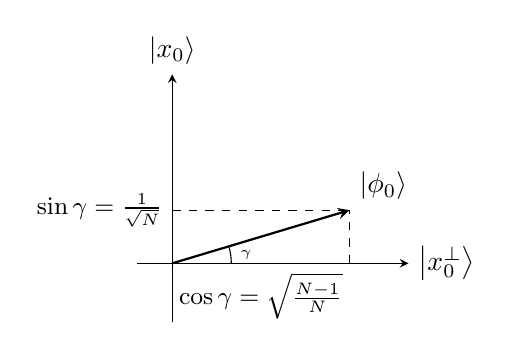
\begin{tikzpicture}[scale=1.5,>=stealth]
  \draw[->] (-0.3,0) -- (2,0) node[right] {$\ket{x_0^\perp}$};
  \draw[->] (0,-0.5) -- (0,1.6) node[above] {$\ket{x_0}$};
  \draw[->,thick] (0,0) -- (1.5,0.45) node[above right] {$\ket{\phi_0}$};
  \draw[dashed] (0,0.45) -- (1.5,0.45);
  \draw[dashed] (1.5,0) -- (1.5,0.45);
  \node[left] at (0,0.45) {\small $\sin\gamma = \frac{1}{\sqrt N}$};
  \node[below] at (0.75,0) {\small $\cos\gamma = \sqrt{\frac{N-1}{N}}$};
  \draw (0.5,0) arc (0:16.7:0.5) node[midway,right] {\tiny$\gamma$};
\end{tikzpicture}
\end{minipage}\hfill
\begin{minipage}{0.55\textwidth}
Since the Grover operator is composed of rotations around $\ket{x_0}$ and $\ket{\phi_0}$, and both are in the plane spanned by $\{\ket{x_0},\ket{x_0^\perp}\}$, we can analyze geometrically in this plane.
\end{minipage}

\medskip
$W := \operatorname{span}\{\ket{x_0},\ket{x_0^\perp}\}\ \to\ G_f: W\to W$.

If the state is $\ket{\phi_\theta} = \sin\theta\ket{x_0} + \cos\theta\ket{x_0^\perp}$, $G_f$ acts on the angle $\theta$ s.t.\ $\theta\mapsto 2\gamma+\theta$.

% geometric steps of one Grover iteration (gamma = 12 deg, theta = 30 deg)
\newcommand{\groveraxes}{%
  \draw[->] (-1.4,0) -- (1.6,0) node[right] {\small$\ket{x_0^\perp}$};
  \draw[->] (0,-1.3) -- (0,1.4) node[above] {\small$\ket{x_0}$};
  \draw[->,gray] (0,0) -- (12:1.3) node[above,font=\tiny] {$\ket{\phi_0}$};}
\begin{center}
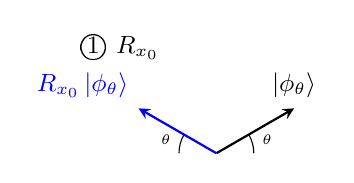
\begin{tikzpicture}[scale=0.95,>=stealth]
  \node at (-1.3,1.4) {\small\textcircled{1} $R_{x_0}$};
  \groveraxes
  \draw[->,thick] (0,0) -- (30:1.2) node[above] {\small$\ket{\phi_\theta}$};
  \draw[->,thick,blue] (0,0) -- (150:1.2) node[above left] {\small$R_{x_0}\ket{\phi_\theta}$};
  \draw (0.5,0) arc (0:30:0.5); \node at (15:0.7) {\tiny$\theta$};
  \draw (-0.5,0) arc (180:150:0.5); \node at (165:0.7) {\tiny$\theta$};
\end{tikzpicture}
\hspace{0.3cm}
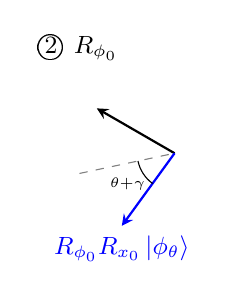
\begin{tikzpicture}[scale=0.95,>=stealth]
  \node at (-1.3,1.4) {\small\textcircled{2} $R_{\phi_0}$};
  \groveraxes
  \draw[->,thick] (0,0) -- (150:1.2);
  \draw[->,thick,blue] (0,0) -- (234:1.2) node[below] {\small$R_{\phi_0}R_{x_0}\ket{\phi_\theta}$};
  \draw[dashed,gray] (192:1.3) -- (12:0.01);
  \draw (234:0.5) arc (234:192:0.5); \node at (213:0.75) {\tiny$\theta{+}\gamma$};
\end{tikzpicture}
\hspace{0.3cm}
\begin{tikzpicture}[scale=0.95,>=stealth]
  \node at (-1.3,1.4) {\small\textcircled{3} $(-)$};
  \groveraxes
  \draw[->,dashed] (0,0) -- (234:1.2);
  \draw[->,thick,blue] (0,0) -- (54:1.2) node[above] {\small$\theta+2\gamma$};
  \draw (0.5,0) arc (0:54:0.5);
\end{tikzpicture}
\end{center}

For $k\in\mathbb{N}$:
\begin{align*}
\ket{\phi_k} = (G_f)^k\ket{\phi_0} = \sin(\gamma + 2k\gamma)\ket{x_0} + \cos(\gamma+2k\gamma)\ket{x_0^\perp}.
\end{align*}
The probability to get outcome $x_0$ is
\[
P_r = \bigl|\braket{\phi_r}{x_0}\bigr|^2 = \bigl|\sin[\gamma(1+2r)]\bigr|^2.
\]
If we want $P_r\approx1$, then
\[
\gamma(1+2r) \approx \frac\pi2 + m\pi
\quad\Rightarrow\quad
r = \frac{2m+1}{4\gamma}\pi - \frac12 = \frac{(2m+1)\pi}{4\arcsin\bigl(\frac{1}{\sqrt N}\bigr)} - \frac12.
\]
If we assume $N\gg1$, $\arcsin\bigl(\frac{1}{\sqrt N}\bigr) = \frac{1}{\sqrt N} + O\Bigl(\frac{1}{\sqrt N^{\,3}}\Bigr)$
\[
\Rightarrow\ \boxed{r = \frac\pi4\sqrt N - \frac12 + \underbrace{O(1)}_{\text{round to closest integer}}\in\mathbb{N}}
\]
\[
P_r = \Bigl|\sin\Bigl(\frac\pi2 + O\Bigl(\frac{1}{\sqrt N}\Bigr)\Bigr)\Bigr|^2 = \boxed{1 - O\Bigl(\frac1N\Bigr)}
\]
After a rotation by $\pi$, the overlap with $-\ket{x_0}$ is high.\\
Period: $\Delta r = \frac\pi2\sqrt N + O(1)$.

It can be proven that any quantum algorithm solving the search problem has to query the oracle $\Omega(\sqrt N)$ times\\
$\Rightarrow$ Grover is \textsc{optimal}.

\subsection{Multiple marked elements}

There is a set $S$ of $M>1$ marked elements. The circuit is the same, but
\[
U_f = \id - 2\Pi_S,\qquad \Pi_S = \sum_{x\in S}\ketbra{x}{x},\qquad \ket{S} = \frac{1}{\sqrt M}\sum_{x\in S}\ket{x}.
\]
In the same way as the $M=1$ case, we write
\[
\ket{\phi_0} = \sin\gamma\ket{S} + \cos\gamma\ket{S^\perp},\qquad \sin\gamma = \sqrt{\frac MN}.
\]
After $r$ iterations:
\[
P_r = \bigl|\braket{\phi_r}{S}\bigr|^2 = \sin^2\Bigl((2r+1)\arcsin\sqrt{\frac MN}\Bigr)
\quad\text{and}\quad
\boxed{r\approx\frac\pi4\sqrt{\frac NM}}\qquad M\ll N.
\]
If we don't know $M$, try $M'=1$; if it fails, $M'=2,\dots$\\
The total number of queries is $O(\sqrt N)$.

%======================================================================
\section{Amplitude amplification}

Generalization of Grover's algorithm, with a set of marked elements $S$, $|S|=M$, and we have a heuristic guessing algorithm $A$:
\[
A\ket{0}^{\otimes n} = \sum_{x\in\{0,1\}^n}\alpha_x\ket{x} =: \ket{\psi}.
\]
$P = P^2$ good projector, $\expval{\psi}{P}{\psi} = g$: probability to be in the good state.

The goal is to increase the overlap with the good state, i.e.\ increase $g$.\\
The circuit is the same as Grover, but replacing $H^{\otimes n}$ with $A$:

\begin{center}
\begin{quantikz}
\lstick{$\ket0$} & \gate[4]{A} & \gate[4]{U_f}\gategroup[4,steps=4,style={dashed,rounded corners,inner xsep=3pt},label style={label position=below,anchor=north,yshift=-0.2cm}]{repeat $k$ times} & \gate[4]{A^{-1}} & \gate[4]{-U_0} & \gate[4]{A} & \meter[4]{} & \setwiretype{c} \\
\lstick{$\ket0$} & & & & & & & \setwiretype{c} \\
\setwiretype{n}\lstick{$\vdots$} & & & & & & & \\
\lstick{$\ket0$} & & & & & & & \setwiretype{c}
\end{quantikz}
\end{center}

The good state can be defined as
\[
\ket{g} = \frac{P\ket{\psi}}{\sqrt g},\qquad \ket{g^\perp} = \ket{b} = \frac{(\id-P)\ket{\psi}}{\sqrt{1-g}}.
\]
Here $\sin\gamma = \sqrt g$, $\cos\gamma = \sqrt{1-g}$, and
\[
G_f = -R_{\ket\psi}R_{\ket g},
\]
where $R_{\ket g} = 2P-\id$ is the reflection around $\ket g$, and $R_{\ket\psi} = -A\,U_0A^{-1} = 2\ketbra\psi\psi - \id$ is the reflection about the state $\ket\psi = A\ket{0}^{\otimes n}$.

$\Rightarrow$ Rotation of $2\gamma$ from $\ket\psi$ towards $\ket g$ (same as Grover) in the plane $\ket g,\ket b$.\\
The state after $k$ iterations is
\[
G_f^k\ket\psi = \sin\bigl(\gamma(2k+1)\bigr)\ket g + \cos\bigl(\gamma(2k+1)\bigr)\ket b,
\qquad
\bigl|\braket{\psi_k}{g}\bigr|^2 = \sin^2\bigl(\gamma(2k+1)\bigr).
\]
For small $g$, $\gamma = \arcsin\sqrt g\approx\sqrt g$ $\Rightarrow$ $k\approx\Bigl\lfloor\frac{\pi}{4\sqrt g}\Bigr\rfloor = O\Bigl(\frac{1}{\sqrt g}\Bigr)$\\
$\to$ improvement over $O\bigl(\sqrt{N/M}\bigr)$ if $g > \frac MN$.

Overall circuit size $\approx O\bigl(k(s+n)\bigr)$, with $s$ = circuit size of $f$.
\begin{itemize}
  \item Grover is a.a.\ where the heuristic gives uniform probability ($A = H^{\otimes n}$).
\end{itemize}

%======================================================================
\section{Quantum Fourier transform}

$\Hil = \CC^d$ ($d = 2^n$), \quad $\omega_d := e^{\frac{2\pi i}{d}}$.\\
Define
\[
\mathrm{QFT}_d = \frac{1}{\sqrt d}\sum_{j=0}^{d-1}\sum_{k=0}^{d-1}\omega^{jk}\ketbra{j}{k},
\qquad
\mathrm{QFT}_d\ket{k} = \frac{1}{\sqrt d}\sum_{j=0}^{d-1}e^{2\pi i\frac{k\cdot j}{d}}\ket{j}.
\]
This is unitary: $\mathrm{QFT}^\dagger\mathrm{QFT} = \id$.

Binary notation: $y = y_0 + 2y_1 + \dots + 2^{n-1}y_{n-1} = \sum_{k=0}^{n-1}2^ky_k$, \quad $\ket y = \ket{y_{n-1}}\ket{y_{n-2}}\cdots\ket{y_0}$.\\
Binary fraction: $0.x_jx_{j-1}\dots x_0 = \sum_{k\le j}\frac{x_k}{2^{j-k+1}}$.

We can derive another representation for the action of QFT on a state:
\begin{align*}
\mathrm{QFT}_d\ket{x} &= \frac{1}{\sqrt d}\sum_{y=0}^{d-1}e^{\frac{2\pi i}{d}x\cdot\left(\sum_{k=0}^{n-1}2^ky_k\right)}\ket{y_{n-1}}\cdots\ket{y_0}\\
&= \bigotimes_{j=1}^{n}\Bigl(\frac{1}{\sqrt2}\sum_{y_{n-j}=0}^{1}e^{\frac{2\pi i}{2^j}x\,y_{n-j}}\ket{y_{n-j}}\Bigr)\\
&= \bigotimes_{j=1}^{n}\frac{1}{\sqrt2}\Bigl(\ket0 + e^{2\pi i\,0.x_{j-1}\dots x_0}\ket1\Bigr)\\
&= \ket{0.x_0}\ket{0.x_1x_0}\cdots\ket{0.x_{n-1}\dots x_0}
\end{align*}
where $\ket{0.b} := \frac{1}{\sqrt2}\bigl(\ket0 + e^{2\pi i\,0.b}\ket1\bigr)$. Side note: for $y_{n-j}=1$ the phase is $2\pi i\,\frac{x}{2^j} = \sum_k 2\pi i\,x_k2^{k-j}$; the terms with $k\ge j$ are integer multiples of $2\pi i$ and drop out, the terms with $k<j$ give $0.x_{j-1}\dots x_0$.

We can implement an efficient circuit for $\mathrm{QFT}_d$ ($d=2^n$) recursively.\\
$n=1\ \to\ \mathrm{QFT}_2 = H$.
\[
R_k := \operatorname{diag}\bigl(1, e^{\pi i/2^k}\bigr) = \operatorname{diag}\bigl(1, e^{2\pi i\,0.\overbrace{\scriptstyle 0\dots0}^{k}x}\bigr)
\]
We apply a sequence of controlled-$R_k$ to the next qubit:

\begin{center}
\begin{quantikz}
\lstick{$\ket{x_1}$} & \gate{H} & \gate{R_1} & & & \swap{1} & \rstick{$\ket{y_1} = \ket{0.x_0}$}\\
\lstick{$\ket{x_0}$} & & \ctrl{-1} & \gate{H}\gategroup[1,steps=1,style={dashed,inner sep=3pt},label style={label position=below,anchor=north,yshift=-0.2cm}]{$\mathrm{QFT}_1$} & & \targX{} & \rstick{$\ket{y_0} = \ket{0.x_1x_0}$}
\end{quantikz}
\end{center}

\begin{center}
\begin{quantikz}[row sep={0.8cm,between origins}]
\lstick{$\ket{x_{n-1}}$} & \gate{H} & \gate{R_1} & \ \ldots\ & \gate{R_{n-1}} & & \rstick{$\ket{0.x_{n-1}\dots x_0}$}\\
\lstick{$\ket{x_{n-2}}$} & & \ctrl{-1} & \ \ldots\ & & \gate[3]{\mathrm{QFT}_{n-1}} & \\
\setwiretype{n}\lstick{$\vdots$} & & & & & & \\
\lstick{$\ket{x_0}$} & & & \ \ldots\ & \ctrl{-3} & & \rstick{$\ket{0.x_0}$}
\end{quantikz}
\end{center}
In the end we have to swap to get the right order: $\ket{0.x_0}\ket{0.x_1x_0}\cdots\ket{0.x_{n-1}\dots x_0}$.

Total number of gates: $n + (n-1) + \dots = \frac{n(n+1)}{2} = O(n^2)$.
\begin{itemize}
  \item $\mathrm{QFT}\ket{0}^{\otimes n} = H^{\otimes n}\ket0^{\otimes n} = \frac{1}{\sqrt d}\sum_{k=0}^{d-1}\ket k$,\\
  but $\mathrm{QFT}\ket1\otimes\ket0^{\otimes n-1} = \frac{1}{\sqrt d}\sum_{k=0}^{d-1}(-1)^k\ket k \neq H^{\otimes n}\ket1\otimes\ket0^{\otimes n-1}$.
  \item Generalized gates:
  \begin{align*}
  Z_d &= \sum_{j=0}^{d-1}e^{2\pi i\frac jd}\ketbra jj &&\to \text{eigenstates } \ket j,\ \lambda = e^{2\pi i\frac jd}\\
  X_d &= \sum_{j=0}^{d-1}\ketbra{j\oplus1}{j} &&\to \text{eigenstates } \mathrm{QFT}_d\ket j,\ \lambda = e^{-\frac{2\pi i}{d}j}
  \end{align*}
  $\Rightarrow$ Generalized $H_d\ket x = \frac{1}{\sqrt d}\sum_{y=0}^{d-1}e^{2\pi i\frac{xy}{d}}\ket y$, because it takes eigenvectors of $Z_d$ to eigenvectors of $X_d$.
  \[
  (\id\otimes\mathrm{QFT}_d^\dagger)\,CZ_d\,(\id\otimes\mathrm{QFT}_d)\ket x\ket j = \ket x\ket{j+x\ (\mathrm{mod}\ d)}
  \]
  (if $d=2$: $H_2\,CZ\,H_2 = \mathrm{CNOT}$)
  \item $\boxed{\frac1d\sum_{j=0}^{d-1}e^{-\frac{2\pi i}{d}jk} = \delta_{0,k\,(\mathrm{mod}\ d)}}$ \qquad
  $\sum_{x=0}^{2^n-1}(-1)^{x\cdot y}\neq0 \iff y=0$
\end{itemize}

%======================================================================
\section{Quantum phase estimation}

Given a unitary $U$ and $\ket\varphi$: $U\ket\varphi = e^{2\pi i\varphi}\ket\varphi$, $\varphi\in[0,1)$, the goal is to find $\varphi$ to $t$-bit precision:
\[
\varphi = 0.\varphi_{t-1}\varphi_{t-2}\dots\varphi_0 = \sum_{j=1}^t\varphi_{t-j}2^{-j}.
\]
\begin{center}
\begin{quantikz}[row sep={0.8cm,between origins}]
\lstick[4]{$t$}\lstick{$\ket0$} & \gate{H} & \ctrl{4} & & \ \ldots\ & & \gate[4]{\mathrm{QFT}^\dagger} & \rstick{$\ket{\varphi_0}$}\\
\lstick{$\ket0$} & \gate{H} & & \ctrl{3} & \ \ldots\ & & & \rstick{$\ket{\varphi_1}$}\\
\setwiretype{n}\lstick{$\vdots$} & \vdots & & & & & & \\
\lstick{$\ket0$} & \gate{H} & & & \ \ldots\ & \ctrl{1} & & \rstick{$\ket{\varphi_{t-1}}$}\\
\lstick{$\ket\varphi$} & \qwbundle{} & \gate{U_{t-1}} & \gate{U_{t-2}} & \ \ldots\ & \gate{U_0} & & \rstick{$\ket\varphi$}
\end{quantikz}
\end{center}
We apply controlled $U_k = U^{2^k}$ to create the state $\ket{0.\varphi_0}\ket{0.\varphi_1\varphi_0}\cdots\ket{0.\varphi_{t-1}\dots\varphi_0}$ and then apply the inverse QFT $\to\ket{\varphi_0}\ket{\varphi_1}\cdots\ket{\varphi_{t-1}}$.

\begin{minipage}{0.3\textwidth}
\begin{quantikz}
\lstick{$\ket+$} & \ctrl{1} & \\
\lstick{$\ket\varphi$} & \gate{U} &
\end{quantikz}
\end{minipage}
\begin{minipage}{0.65\textwidth}
\begin{align*}
\ket+ &\to \tfrac{1}{\sqrt2}\bigl(\ket0\ket\varphi + U\ket1\ket\varphi\bigr)
= \tfrac{1}{\sqrt2}\bigl(\ket0 + e^{2\pi i\varphi}\ket1\bigr)\ket\varphi\\
&= R_z(\varphi)\ket+ = \ket{0.\varphi_{t-1}\dots\varphi_0}
\end{align*}
\end{minipage}

$\Rightarrow R_z(2^k\varphi) = U^{2^k}$ and $R_z(2^k\varphi)\ket+ = \ket{0.\varphi_{t-k-1}\dots\varphi_0}$.

For an arbitrary $\varphi\in[0,1)$, if we want $n$-bit precision with probability $1-\varepsilon$:
\[
t = n + \Bigl\lceil\log\Bigl(2+\frac{1}{2\varepsilon}\Bigr)\Bigr\rceil.
\]
In the general case, $O(2^t)$ gates are required for implementing QPE.

%======================================================================
\section{Order finding}

For $a$ coprime ($\gcd(N,a)=1$) to $N\le2^n$, consider the unitary
\[
U\ket x = \begin{cases}\ket{a\cdot x\ (\mathrm{mod}\ N)} & x\le N-1\\ \ket x & \text{else}\end{cases}
\]
It is unitary, because $U_a^r\ket x = \ket{\overbrace{a^r}^{=1\,(\mathrm{mod}\,N)}x\ \mathrm{mod}\ N} = \ket x$.\\
The goal is to find the \textsc{order} $r$: $a^r\bmod N = 1$ (smallest $r$).

Eigenvectors of $U$ are the states

\[
\ket{\varphi^{(s)}} = \frac{1}{\sqrt r}\sum_{k\in\mathbb{Z}_r}e^{-2\pi i\frac{sk}{r}}\ket{a^k\ (\mathrm{mod}\ N)}
\qquad\text{with eigenvalues } \lambda_s = e^{+2\pi i\frac sr}.
\]
We use QPE to find $\lambda_s$ (that is $\frac sr$).\\
We don't know $\ket{\varphi^{(s)}}$, but $\ket1$ is an equal superposition of all $\ket{\varphi^{(s)}}$, $s\in\mathbb{Z}_r$:
\[
\ket1 = \frac{1}{\sqrt r}\sum_{s\in\mathbb{Z}_r}\ket{\varphi^{(s)}}.
\]
Let $\bigl(\frac sr\bigr) = \sum_{k<t}\bigl(\frac sr\bigr)_k2^{-k}$ (binary rep.). At the end of QPE we have the state
\[
\sum_{s<r}\frac{1}{\sqrt r}\Ket{\bigl(\tfrac sr\bigr)_0}\Ket{\bigl(\tfrac sr\bigr)_1}\cdots\Ket{\bigl(\tfrac sr\bigr)_{t-1}}\ket{\varphi^{(s)}}.
\]
If we measure the first $t$ qubits we collapse the superposition to a random $s$ with equal probability $1/r$.\\
$\to$ We get an approximation up to $t$ bits of precision of $s/r$!

Then we use the classical \textsc{continued fraction algorithm}: if the output $\varphi'$ satisfies $\bigl|\varphi' - \frac sr\bigr| \le \frac{1}{2r^2}$, CF returns $\frac sr$ in lowest terms; running QPE twice (independent outputs $\varphi,\varphi'$) and taking the l.c.m.\ of the two denominators gives $r$ with probability $\ge\frac14$ $\to O(n^3)$.\\
To satisfy the bit precision, $t = 2n+1+\bigl\lceil\log\bigl(2+\frac{1}{2\varepsilon}\bigr)\bigr\rceil$.

The last problem is how to build $2^{t-1}$ C-$U$ gates. Fortunately, there is a smart way:
\[
U_a^{2^k}: x\mapsto a^{2^k}x\ (\mathrm{mod}\ N).
\]
We compute $z_k = a^{2^k}\bmod N = z_{k-1}^2\bmod N$ recursively with Boolean circuits, then implement $(y,x)\mapsto(y, z_k^yx\bmod N)$ as a controlled quantum gate $\to O(t\cdot n^2)$.

$\Rightarrow$ Overall complexity is $\boxed{O(n^3)}$!

%======================================================================
\section{Shor's algorithm}

The task is, given a number $N$ ($n$ bit), find a factor $q<N$.\\
Best known classical algorithm (number field sieve) $\to e^{O(n^{1/3}(\log n)^{2/3})}$, superpolynomial in $n$.
\begin{enumerate}
  \item Pick a random $a$: $\gcd(a,N)=1$ (if we see $\gcd\neq1$, it's a factor. We can check efficiently with Euclid's algorithm).
  \item Find the order of $a$, $r$, defined as the smallest that satisfies $a^r = 1\ (\mathrm{mod}\ N)$ (QPE order finding, $O(n^3)$).\\
  With high probability ($\ge\frac12$), $r$ is even and neither $(a^{r/2}+1)$ nor $(a^{r/2}-1)$ is a multiple of $N$:
  \[
  a^r - 1 = 0\ (\mathrm{mod}\ N) = \underbrace{(a^{r/2}+1)}_{\neq0\ \mathrm{mod}\ N\text{ with }p\ge\frac12}\ \overbrace{(a^{r/2}-1)}^{\substack{\neq0\ \mathrm{mod}\ N\text{ 'cause }r\text{ is the}\\ \text{smallest with this property}}}
  \]
  $\Rightarrow (a^{r/2}+1)$ must share factors with $N$.
  \item Compute $\gcd\bigl((a^{r/2}+1),N\bigr) = p$, then $q = \frac Np$ is the output (or simply $p$).
\end{enumerate}
$\to$ Including all the checks during the algorithm, $O(n^3)$.

%======================================================================
\section{Density operators}

Consider an ensemble $\{(p_x,\ket{\varphi_x})\}$ $\to$ density operator $\rho := \sum_xp_x\ketbra{\varphi_x}{\varphi_x}$.
\begin{itemize}
  \item Probability given $x$ is the Born rule $\expval{\varphi_x}{\Pi_y}{\varphi_x}$. Average over all $x$:
  \[
  \Pr[\Pi_y] = \sum_xp_x\expval{\varphi_x}{\Pi_y}{\varphi_x} = \Tr\Bigl[\Pi_y\Bigl(\sum_xp_x\ketbra{\varphi_x}{\varphi_x}\Bigr)\Bigr] = \Tr(\Pi_y\rho)
  \]
  \item $\Tr[\rho] = 1$
  \item $\rho\ge0 \iff \forall\ket\psi\in\Hil$, $\expval\psi\rho\psi\ge0$ (that is, positive semi-definite), and $\rho = \rho^\dagger$
\end{itemize}
The ensemble is NOT unique ($\{(\frac12,\ket0),(\frac12,\ket1)\}$ and $\{(\frac12,\ket+),(\frac12,\ket-)\}$ both have $\rho = \id/2$).

\subsection{Marginal states}

Bipartite state $\ket\psi_{AB}\in\Hil_A\otimes\Hil_B$. We can get the marginal state $\rho_A$ by tracing out $B$. We call $\Tr_B$ the \textsc{partial trace}:
\[
\rho_A = \Tr_B\bigl(\ketbra\psi\psi_{AB}\bigr)\ \to\ \text{always a valid state.}
\]
If $\Pi_y = \Pi_A\otimes\id_B$: \quad $\Pr(\Pi_y) = \Tr_A\bigl[\Pi_A\Tr_B\bigl(\ketbra\psi\psi_{AB}\bigr)\bigr]$.

Entangled states have mixed marginal states.\\
We call \textsc{purification} of $\rho_A$ a $\ket\psi_{AB}$, for some $\Hil_B$, s.t.\ $\rho_A = \Tr_B\bigl(\ketbra\psi\psi_{AB}\bigr)$.

%======================================================================
\section{Quantum channels}

Closed system: $\ket\psi\mapsto U\ket\psi$.\\
Open system: interacts with the environment, so we apply closed-system dynamics to system $+$ env.:
\[
\ket\psi_A\otimes\ket0_E\mapsto U_{AE}\bigl(\ket\psi_A\otimes\ket0_E\bigr).
\]
To find a description of the dynamics of $A$, we apply $U_{AE}$ and trace out $E$:
\begin{align*}
\rho_A &= \Tr_E\bigl[U_{AE}\bigl(\ketbra\psi\psi_A\otimes\ketbra00_E\bigr)U_{AE}^\dagger\bigr]\\
&= \sum_{j=0}^{d_E-1}K_A(j)\ketbra\psi\psi_AK_A(j)^\dagger\\
&= \mathcal N\bigl[\ketbra\psi\psi\bigr]\qquad\textsc{quantum channel}
\end{align*}
$\mathcal N$ is represented by \textsc{Kraus operators} $\{K_A(j)\}_j$.
\begin{itemize}
  \item $\sum_jK_j^\dagger K_j = \id \iff \Tr\bigl[\mathcal N[M]\bigr] = \Tr(M)$ \quad$\to$ \textsc{trace preserving}
  \item $\mathcal N_A\otimes\id_B[\rho_{AB}]\ge0$ \quad$\to$ \textsc{completely positive}
\end{itemize}
\[
K(j) := {}_E\!\bra{j}U_{AE}\ket0_E
\]
\begin{itemize}[label=$\to$]
  \item Pauli channel: $\rho\mapsto\sum_{j=0}^3p_j\sigma_j\rho\sigma_j^\dagger$, \quad $K(j) = \sqrt{p_j}\,\sigma_j$
  \item Bit flip: $\rho\mapsto(1-p)\rho + p\,\sigma_x\rho\sigma_x$; \quad $K(0) = \sqrt{1-p}\,\id$, $K(1) = \sqrt p\,\sigma_x$
  \item Dephasing: $\rho\mapsto(1-p)\rho + p\,\sigma_z\rho\sigma_z$; \quad $K(0) = \sqrt{1-p}\,\id$, $K(1) = \sqrt p\,\sigma_z$
  \item Amplitude damping: with prob.\ $\gamma$, $\ket1\to\ket0$:
  \[
  K(0) = \ketbra00 + \sqrt{1-\gamma}\,\ketbra11,\qquad K(1) = \sqrt\gamma\,\ketbra01
  \]
\end{itemize}

Measurement is a channel too: $K(j) = \Pi_j\otimes\ket j$.
\[
\rho_a\mapsto\rho_{ax} = \sum_j\underbrace{\bigl(\Pi_j\rho_a\Pi_j\bigr)}_{\text{post-measurement state}}\otimes\overbrace{\bigl(\ketbra jj\bigr)_x}^{\text{outcome}}
\]
\begin{align*}
\rho_a &= \Tr_x[\rho_{ax}] = \sum_j\Pi_j\rho_a\Pi_j &&\text{non-selective measurement}\\
\rho_x &= \Tr_a[\rho_{ax}] = \sum_j\underbrace{\Tr[\Pi_j\rho_a]}_{=p_j}\ketbra jj &&\to\text{probability distribution of outcomes}
\end{align*}
This works for arbitrary Kraus operators $\{K_j\}$: $\Lambda_j = K_j^\dagger K_j$ generalizes projective measurement.

%======================================================================
\section{Repetition code}

In the classical case:
\[
\text{encode}\ \begin{array}{l}0\to000\\1\to111\end{array}
\ \overset{\text{noise}}{\rightsquigarrow}\
\underset{\text{(majority vote)}}{\text{decode}}\ \begin{array}{l}011\to1\\010\to0\end{array}
\]
If an error occurs with probability $p$, and we can correct single errors, the fail probability is $p^2(3-2p)$, and if $p<\frac12$, there's improvement.

In the quantum case, if we want to correct \textsc{bit flips}:
\begin{description}[leftmargin=!,labelwidth=3.2em]
  \item[enc:] $\ket\psi = \alpha\ket0+\beta\ket1\to\alpha\ket{000}+\beta\ket{111}$, \quad $\ket0_L = \ket{000}$, $\ket1_L = \ket{111}$.\\
  Logical operators: $X_L = XXX$, $Z_L = ZZZ$; \quad $Z_L\ket1_L = -\ket1_L$, $X_L\ket0_L = \ket1_L$.
  \item[noise:] $\langle X\id\id,\ \id X\id,\ \id\id X\rangle\to$ single-qubit bit flip
  \item[dec:] \textsc{syndrome} measurements of the observables
  \[
  S_1 = \id ZZ = P_0 - P_1,\qquad S_2 = Z\id Z,
  \]
  where $P_0 = \id\otimes\bigl(\ketbra{00}{00}+\ketbra{11}{11}\bigr)$, $P_1 = \id\otimes\bigl(\ketbra{01}{01}+\ketbra{10}{10}\bigr)$.
\end{description}
$S_1$ and $S_2$ have to commute with $X_L,Z_L$, otherwise we would get information about the state and collapse it.\\
We get measurement outcomes $(-1)^{s_1},(-1)^{s_2}$ $\rightsquigarrow$ based on this result we apply a correction.

\begin{center}
\begin{quantikz}[row sep={0.75cm,between origins}]
\lstick{$\ket\psi$} & \ctrl{1}\gategroup[3,steps=2,style={draw=none},label style={label position=below,anchor=north,yshift=-0.1cm}]{enc} & \ctrl{2} & \slice{$\ket\psi_L$} & \gate[3,style={fill=gray!15,rounded corners,dashed}]{\text{noise}} & & & \ctrl{4} & & \gate[3]{U}\gategroup[5,steps=1,style={draw=none},label style={label position=above,anchor=south}]{recovery} & \\
\lstick{$\ket0$} & \targ{} & & & & \ctrl{2} & & & & & \\
\lstick{$\ket0$} & & \targ{} & & & & \ctrl{1} & & \ctrl{2} & & \\
\setwiretype{n} & & & & \push{\ket0} & \targ{}\setwiretype{q} & \targ{} & & & \meter{} \rstick{$s_1$} & \setwiretype{n} \\
\setwiretype{n} & & & & \push{\ket0} & \setwiretype{q} & & \targ{} & \targ{} & \meter{} \rstick{$s_2$} & \setwiretype{n}
\end{quantikz}
\end{center}
Ancilla 1 measures $S_1 = \id ZZ$ (CNOTs from qubits 2,3), ancilla 2 measures $S_2 = Z\id Z$ (CNOTs from qubits 1,3); a classical function $f(s_1,s_2)$ of the outcomes selects the recovery $U$.

\begin{center}
\begin{tabular}{c|c}
\textsc{Syndrome} & $U$\\ \hline
$(1,1)$ & $\id\id\id$\\
$(1,-1)$ & $X\id\id$\\
$(-1,1)$ & $\id X\id$\\
$(-1,-1)$ & $\id\id X$
\end{tabular}
\qquad It fails if 2 or more errors occurred.
\end{center}

It can correct any single-qubit Kraus operator $K = c_0\id + c_1X$, $c_0,c_1\in\CC$.

If we want to protect against \textsc{phase flip} errors, we use $H$ to map $X\leftrightarrow Z$:
\[
\ket+\to\ket{+++},\qquad\ket-\to\ket{---},\qquad X_L = ZZZ,\quad Z_L = XXX\ (\text{equivalently } X\id\id)
\]
and measure $S_1 = \id XX$, $S_2 = X\id X$.\\
Same circuit, but with $H$ gates on the data qubits after encoding and before decoding.

%======================================================================
\section{Shor's 9-qubit code}

The idea is to concatenate encoders.

\begin{minipage}{0.6\textwidth}
\centering
\begin{quantikz}[row sep={0.55cm,between origins},column sep=0.25cm]
 & \gate{H} & \ctrl{3} & \ctrl{6} & \gate{H} & \ctrl{1} & \ctrl{2} & \\
\setwiretype{n} & & & & \push{\ket0} & \targ{}\setwiretype{q} & & \\
\setwiretype{n} & & & & \push{\ket0} & \setwiretype{q} & \targ{} & \\
\lstick{$\ket0$} & & \targ{} & & \gate{H} & \ctrl{1} & \ctrl{2} & \\
\setwiretype{n} & & & & \push{\ket0} & \targ{}\setwiretype{q} & & \\
\setwiretype{n} & & & & \push{\ket0} & \setwiretype{q} & \targ{} & \\
\lstick{$\ket0$} & & & \targ{} & \gate{H} & \ctrl{1} & \ctrl{2} & \\
\setwiretype{n} & & & & \push{\ket0} & \targ{}\setwiretype{q} & & \\
\setwiretype{n} & & & & \push{\ket0} & \setwiretype{q} & \targ{} &
\end{quantikz}
\end{minipage}\hfill
\begin{minipage}{0.35\textwidth}
\centering
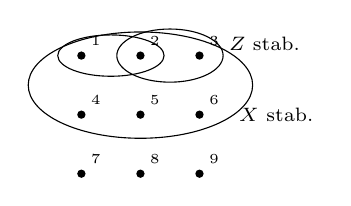
\begin{tikzpicture}[scale=0.75]
  \foreach \i in {1,...,9} {
    \pgfmathsetmacro{\x}{mod(\i-1,3)}
    \pgfmathsetmacro{\y}{-floor((\i-1)/3)}
    \fill (\x,\y) circle (2pt) node[above right,font=\tiny] {\i};
  }
  \draw (0.5,0) ellipse (0.9 and 0.35);
  \draw (1.5,0) ellipse (0.9 and 0.45);
  \node[font=\scriptsize] at (3.1,0.2) {$Z$ stab.};
  \draw (1,-0.5) ellipse (1.9 and 0.9);
  \node[font=\scriptsize] at (3.3,-1) {$X$ stab.};
\end{tikzpicture}
\end{minipage}

The first $H$ makes the encoder map $\ket\pm\mapsto\ket{\bar\pm}$ (below); without it one gets the usual convention $\ket0_L = \ket{\hat+}^{\otimes3}$, $\ket1_L = \ket{\hat-}^{\otimes3}$, with the roles of $\bar X$ and $\bar Z$ exchanged.

\begin{align*}
\ket+ &\to \ket{+++} \to \bigl(\ket{000}+\ket{111}\bigr)^{\otimes3} = \ket{\bar+}, \qquad \bigl(\ket{000}+\ket{111}\bigr) = \ket{\hat+}\\
\ket- &\to \ket{---} \to \bigl(\ket{000}-\ket{111}\bigr)^{\otimes3} = \ket{\bar-}, \qquad \bigl(\ket{000}-\ket{111}\bigr) = \ket{\hat-}
\end{align*}
\[
\bar X = X_1X_2X_3,\qquad \bar Z = Z_1Z_4Z_7
\]
Syndrome decoding:
\begin{itemize}[label=--]
  \item Measure syndromes for $X$ errors in each block separately: $\underbrace{Z_2Z_3,\ Z_1Z_3}_{123},\ \underbrace{Z_5Z_6,\ Z_4Z_6}_{456},\ Z_8Z_9,\ Z_7Z_9$
  \item Measure syndromes for $Z$ errors: $X_4X_5X_6X_7X_8X_9$, \ $X_1X_2X_3X_7X_8X_9$
\end{itemize}
$\to$ apply corrections.
\begin{itemize}
  \item All syndrome measurement operators commute, and also with the logical operators.
  \item By degeneracy, $Z$-type errors happen only on qubits 1, 4 or 7.
  \item Shor's code corrects every single-qubit error $K = c_0\id + c_1X + c_2Y + c_3Z$, $c_i\in\CC$.
  \item Corrections to be applied are:
  \begin{itemize}[label=$\to$]
    \item for $X$ errors, $X_i$, where $i$ is the qubit with the error;
    \item for $Z$ errors, $(ZZZ)_{\text{block }j}$, where $j$ is the block with the error.
  \end{itemize}
  \item $Z$ errors on the same block are indistinguishable, e.g.\ $\expval{0_L}{Z_1^\dagger Z_2}{0_L} = \expval{1_L}{Z_1^\dagger Z_2}{1_L}\neq0$ $\to$ indistinguishable.\\
  We can find a new basis of errors by diagonalizing the KL matrix $C_{ab}$ given by $\expval{i_L}{E_a^\dagger E_b}{j_L} = \delta_{ij}C_{ab}$.
\end{itemize}

%======================================================================
\section{Quantum error correction}

Given $\Hil_{\text{logical}}\simeq(\CC^2)^{\otimes k}$ and noise channel $\mathcal N(\rho) = \sum_jE_j\rho E_j^\dagger$, we want to find
\[
\text{dec}: \Hil_{\text{phys}}\to\Hil_{\text{log}},\qquad \text{enc}: \Hil_{\text{log}}\to\Hil_{\text{phys}}\qquad\text{s.t.}\quad \text{dec}\circ\mathcal N\circ\text{enc} = \id,
\]
for some $\Hil_{\text{phys}}\simeq(\CC^2)^{\otimes n}$.

Consider a subgroup of the $n$-qubit Pauli group $S = \langle s_1,\dots,s_{n-k}\rangle\subseteq\mathcal P_n$. We call this the \textsc{stabilizer group} and define the codespace as
\[
\Hil_{\text{code}} = \bigl\{\ket\psi\in\Hil_{\text{phys}} : s\ket\psi = \ket\psi\ \forall s\in S\bigr\}.
\]
If $[s_i,s_j] = 0$ $\forall i,j$ and $-\id^{\otimes n}\notin S$: $\dim(\Hil_{\text{code}}) = 2^k$.

$\to$ Logical operators $\bar X,\bar Z$ s.t.\ $\{\bar X,\bar Z\} = 0$, and they act on the logical basis.

A collection of errors will be correctable if each class leads to a distinct syndrome.

\subsection{Knill--Laflamme conditions}

A code $C$, $\Hil_C$ corrects $\mathcal N(\rho) = \sum_{j=1}^mE_j\rho E_j^\dagger$
\[
\iff \expval{\psi}{E_i^\dagger E_j}{\psi'} = C_{ij}\braket{\psi}{\psi'}\qquad\forall\psi,\psi'\in\Hil_{\text{code}},\ C_{ij}\in\CC,\ i,j = 1,\dots,m.
\]
There are equivalent statements:
\begin{itemize}
  \item $\expval{\bar k}{E_i^\dagger E_j}{\bar\ell} = \delta_{k\ell}C_{ij}$ for an ONB $\{\ket{\bar k}\}$ of $\Hil_{\text{code}}$
  \item $PE_i^\dagger E_jP = c_{ij}P$ for $P$ the projector onto $\Hil_{\text{code}}$
  \item $\expval{\bar\psi}{E_i^\dagger E_j}{\bar\psi} = c_{ij}$ for all $\ket{\bar\psi}\in\Hil_{\text{code}}$
\end{itemize}
Correctability is a property of the set of errors: $\{E_j\}_j$ correctable $\Rightarrow$ $\bigl\{E_j' = \sum_kM_{jk}E_k\bigr\}_j$ correctable ($M_{jk}\in\CC$).

%======================================================================
\section{Stabilizer codes}

Specify the stabilizer group $S\subseteq\mathcal P_n$:
\[
\Hil_{\text{code}} = \bigl\{\ket\psi : s\ket\psi = \ket\psi\ \forall s\in S\bigr\}.
\]
Syndrome decoding $\to$ measure the stabilizer generators and get syndromes $t_1,\dots,t_m$, then apply Pauli corrections.
\begin{itemize}
  \item Given $S$ and $\{E_i\}_i$, KL are satisfied if $\forall i,j$ either
  \begin{enumerate}[label=\alph*)]
    \item $E_i^\dagger E_j\in S$ \quad$\to$ degenerate
    \item $\exists s\in S: \{s, E_i^\dagger E_j\} = 0$ \quad$\to$ non-degenerate
  \end{enumerate}
\end{itemize}

Since two Pauli operators either commute or anticommute, the only case remaining is that $E$ is not in $S$ but commutes with every $s\in S$ $\to$ not detectable:
\[
\forall s\in S\quad sE\ket\psi = Es\ket\psi = E\ket\psi.
\]
\begin{itemize}
  \item Logical operators in stabilizer codes: $\bar X$ and $\bar Z$ s.t.
  \begin{itemize}
    \item $\bar X^2 = \bar Z^2 = \id$, \ $\{\bar X,\bar Z\} = 0$
    \item $[\bar X,s] = [\bar Z,s] = 0$ $\forall s\in S$
    \item $\bar X,\bar Z\notin S$
  \end{itemize}
\end{itemize}
We define the \textsc{distance} of a code as the number of qubits we need to change to go from a codeword to an orthogonal codeword $\to$ the code can correct no more than $\bigl\lfloor\frac{d-1}{2}\bigr\rfloor$ errors.

Examples are the Shor code, Steane code, surface code, 5-qubit code.
\begin{itemize}
  \item $V_S$ (codespace) is the intersection of the subspaces fixed by each operator $s$, and it's a subspace itself.
  \item $\Tr(s_1) = \Tr(i^kP_1\otimes\dots\otimes P_n) = i^k\prod_j\Tr(P_j) = 0$, because $\Tr(X) = \Tr(Y) = \Tr(Z) = 0$\\
  $\Rightarrow$ $2^{n-1}$ $+1$ eigenvalues, $2^{n-1}$ $-1$ eigenvalues $\to$ $s_1$ splits the $2^n$-dim space in half.
  \item To find logical states, start with a ``seed'' that satisfies the logical $Z_L$ condition, then apply the projector onto the $+1$ eigenstate of all stabilizers:
  \[
  \tfrac{1}{2}(\id + s_1)\cdots\tfrac{1}{2}(\id + s_{n-k})\underbrace{\ket{00\dots0}}_{\text{seed}}\quad\text{(then normalize)}
  \]
\end{itemize}

%======================================================================
\section{Stabilizer formalism}

To avoid calculations in Dirac/matrix notation, we specify the state via its stabilizers, and update them after gates or measurements.

\textsc{Gate operation} $U$: if $\ket\psi$ is stabilized by $S_k$, then $U\ket\psi$ is stabilized by $US_kU^\dagger$\\
$\to$ from this we get gate propagation rules ($SU = U(U^\dagger SU)$).

\newcommand{\eqs}{\ \ =\ \ }
\begin{center}
\renewcommand{\arraystretch}{1.2}
\begin{tabular}{l@{\qquad}l}
\fbox{CNOT} &
\begin{quantikz}[column sep=0.3cm,row sep={0.6cm,between origins}]
\push{X} & \ctrl{1} & \\ & \targ{} &
\end{quantikz}\eqs
\begin{quantikz}[column sep=0.3cm,row sep={0.6cm,between origins}]
& \ctrl{1} & \push{X} \\ & \targ{} & \push{X}
\end{quantikz}
\qquad
\begin{quantikz}[column sep=0.3cm,row sep={0.6cm,between origins}]
& \ctrl{1} & \\ \push{X} & \targ{} &
\end{quantikz}\eqs
\begin{quantikz}[column sep=0.3cm,row sep={0.6cm,between origins}]
& \ctrl{1} & \\ & \targ{} & \push{X}
\end{quantikz}
\\[2pt]
&
\begin{quantikz}[column sep=0.3cm,row sep={0.6cm,between origins}]
\push{Z} & \ctrl{1} & \\ & \targ{} &
\end{quantikz}\eqs
\begin{quantikz}[column sep=0.3cm,row sep={0.6cm,between origins}]
& \ctrl{1} & \push{Z} \\ & \targ{} &
\end{quantikz}
\qquad
\begin{quantikz}[column sep=0.3cm,row sep={0.6cm,between origins}]
& \ctrl{1} & \\ \push{Z} & \targ{} &
\end{quantikz}\eqs
\begin{quantikz}[column sep=0.3cm,row sep={0.6cm,between origins}]
& \ctrl{1} & \push{Z} \\ & \targ{} & \push{Z}
\end{quantikz}
\\[4pt]
\fbox{CZ} &
\begin{quantikz}[column sep=0.3cm,row sep={0.6cm,between origins}]
\push{X} & \ctrl{1} & \\ & \control{} &
\end{quantikz}\eqs
\begin{quantikz}[column sep=0.3cm,row sep={0.6cm,between origins}]
& \ctrl{1} & \push{X} \\ & \control{} & \push{Z}
\end{quantikz}
\qquad
\begin{quantikz}[column sep=0.3cm,row sep={0.6cm,between origins}]
& \ctrl{1} & \\ \push{X} & \control{} &
\end{quantikz}\eqs
\begin{quantikz}[column sep=0.3cm,row sep={0.6cm,between origins}]
& \ctrl{1} & \push{Z} \\ & \control{} & \push{X}
\end{quantikz}
\qquad $Z$ unchanged
\\[4pt]
\fbox{$H$} &
\begin{quantikz}[column sep=0.3cm]
\push{X} & \gate{H} &
\end{quantikz}\eqs
\begin{quantikz}[column sep=0.3cm]
& \gate{H} & \push{Z}
\end{quantikz}
\qquad
\begin{quantikz}[column sep=0.3cm]
\push{Z} & \gate{H} &
\end{quantikz}\eqs
\begin{quantikz}[column sep=0.3cm]
& \gate{H} & \push{X}
\end{quantikz}
\\[4pt]
\fbox{$S$} &
\begin{quantikz}[column sep=0.3cm]
\push{X} & \gate{S} &
\end{quantikz}\eqs
\begin{quantikz}[column sep=0.3cm]
& \gate{S} & \push{Y}
\end{quantikz}
\qquad
\begin{quantikz}[column sep=0.3cm]
\push{Z} & \gate{S} &
\end{quantikz}\eqs
\begin{quantikz}[column sep=0.3cm]
& \gate{S} & \push{Z}
\end{quantikz}
\end{tabular}
\end{center}

To analyze a circuit, we start with:
\begin{itemize}
  \item State stabilizers, if specified, e.g.\ $\ket+\to X$; $\ket0\to Z$
  \item Track $(X,Z)$ if the state is unspecified
\end{itemize}
Then we apply the gate rules.

\textsc{Clifford gates}: $\mathcal C_n := \bigl\{U : UgU^\dagger\in\mathcal P_n\ \forall g\in\mathcal P_n\bigr\}$, generated by $(H,S,\mathrm{CNOT})$.\\
If we track $n$ stabilizers, each specified by $2n+2$ bits $\to O(n^2)$ memory used.

\textbf{Gottesman--Knill theorem}: a quantum circuit performing only Clifford gates and measurements in the computational basis can be implemented efficiently on a classical computer.

\textsc{Measurement operation}: Pauli measurement with the stabilizer formalism.
\begin{enumerate}
  \item Check if $M$ commutes with all stabilizers $S_i$.
  \item \begin{itemize}
    \item If $[M,S_i] = 0$ $\forall i$, the measurement outcome is deterministic and the stabilizer list doesn't change.
    \item If $\{M,S_i\} = 0$ for at least one $i$: pick one to be sacrificed, multiply it to every other anticommuting stabilizer, and replace it with $(-1)^aM$, depending on the outcome $a$.
  \end{itemize}
\end{enumerate}

%======================================================================
\section{Fault-tolerant quantum computation}

An operation is defined to be fault-tolerant if a single failure in any of its physical components introduces at most one error per encoded logical block in the output $\to$ \textsc{fault-tolerant gadget}.

The simplest way to construct a FT gate is to implement it \textsc{transversally}, that is, using only independent operations on each of the physical qubits:
\begin{itemize}[label=$\to$]
  \item $H$ for the Steane code: $H^{\otimes7}$
  \item CNOT for the Steane code (bitwise)
\end{itemize}
Errors can spread to the other block, but with the same weight.

\textbf{Eastin--Knill theorem}: no QEC code can have a universal set of gates with transversal implementation\\
$\to$ other options are magic states, code switching, lattice surgery, \dots

\textsc{Syndrome measurement} $\to$ a single error on an ancilla can cause multiple errors in the data\\
$\Rightarrow$ encode the ancilla and perform the measurement transversally.

%======================================================================
\section{Threshold theorem}

Assuming:
\begin{enumerate}
  \item Faults occur independently with probability $p$
  \item QEC can correct 1 error
  \item EC is ideal if: no internal faults and at most 1 input error
  \item EC outputs at most 1 error if: only 1 internal fault and no input errors
\end{enumerate}
The scheme fails if 2 or more errors occur, which is $c\cdot p^2 = O(G^2p^2)$, where $G$ is the number of gates per gadget.\\
There is an improvement if $cp^2<p$, i.e.\ $p<p_{\mathrm{th}} = \frac1c\simeq\frac{1}{G^2}$.

If we are in the condition $p<p_{\mathrm{th}}$ we can improve the logical error rate by \textsc{concatenation}: think of the FT circuit as a new circuit and implement it fault-tolerantly:
\[
p\mapsto cp^2\mapsto c(cp^2)^2 = c^3p^4\mapsto\dots\mapsto c^{2^k-1}p^{2^k} = p_{\mathrm{th}}\Bigl(\frac{p}{p_{\mathrm{th}}}\Bigr)^{2^k}\xrightarrow{k\to\infty}0
\]
If above threshold, the error explodes.
\begin{itemize}
  \item Qubit number scales as $n^k$.
\end{itemize}

%======================================================================
\section{FT error correction by teleportation}

Perform a destructive Bell measurement transversally for an $[n,k]$ code.\\
The Bell measurement is performed bitwise: $X_{A,\alpha}\otimes X_{B,\alpha}$, $Z_{A,\alpha}\otimes Z_{B,\alpha}$ measured for $\alpha = 1,\dots,n$ (can be done by CNOT, then $X$ on control and $Z$ on target).
\begin{itemize}[label=$\to$]
  \item can reconstruct the encoded measurement by multiplying the right outcomes
  \item can extract the syndrome measurement from the same values
\end{itemize}
Then we apply the teleportation protocol: Bell measurement between $A$ and $B$, then correction with logical $\bar X_L,\bar Z_L$ on $C$ to teleport the state that was in $A$.

%======================================================================
\section{FT $\pi/8$ gate}

\begin{center}
\begin{quantikz}
\lstick{$\ket0$} & \gate{H}\gategroup[1,steps=2,style={dashed,rounded corners,inner sep=3pt}]{} & \gate{T} & \slice{$\ket\xi_L$} & \ctrl{1} & \gate{SX} & \rstick{$T\ket\psi$}\\
\lstick{$\ket\psi$} & & & & \targ{} & \meter{}\wire[u][1]{c} &
\end{quantikz}
\qquad
$T = \begin{bmatrix}1 & 0\\ 0 & e^{i\frac\pi4}\end{bmatrix}$
\end{center}
This is a FT implementation of $T$ for the Steane code, assuming we can prepare fault-tolerantly the state $\ket\xi_L = T_LH_L\ket0_L$ and perform FT measurements (because $S$, $X$, CNOT can be implemented transversally with the Steane code).

How to prepare $\ket\xi_L$: since $Z_L\ket0_L = \ket0_L$, then $\ket\xi_L$ will be stabilized by
\[
T_LH_LZ_LH_LT_L^\dagger = T_LX_LT_L^\dagger = e^{-i\frac\pi4}S_LX_L
\]
$\Rightarrow$ Measure $e^{-i\frac\pi4}SX$:
\begin{itemize}
  \item If we get $+1$, we have prepared $\ket\xi_L$.
  \item If we get $-1$, we are in the state $T_LH_L\ket1_L$:
  \[
  T_LH_L\ket1_L = T_LH_LX_L\ket0_L = T_L(H_LX_LH_L)H_L\ket0_L = T_LZ_LH_L\ket0_L = Z_LT_LH_L\ket0_L
  \]
  $\to$ apply $Z_L$ to the final state.
\end{itemize}

\end{document}
